\documentclass{beamer}
\usetheme{Madrid}
\usecolortheme{beaver}
\usepackage{graphicx}
\graphicspath{ {/home/nithin/Pictures/Screenshots} }

%Information to be included in the title page:
\title{Maths Bootcamp}
\author{Anonymous}
\institute{Overleaf}
\date{\today}

\begin{document}

\frame{\titlepage}

\section{Geometry}
\subsection{}
\section{Congruent Triangles}
\section{Similarity }
\subtitle{Algebra}
\subtitle{Probability}

\begin{frame}{Definition of Percentage}
    \begin{itemize}
        \item A \textbf{percentage} is a way of expressing a number as a fraction of 100.
        \item It is denoted by the symbol 
        \item The formula to calculate a percentage is:
        $$
        \text{Percentage} = \left( \frac{\text{Part}}{\text{Whole}} \right) \times 100
        $$
        \item Example: If you score 45 out of 60 on a test, the percentage is:
      $$  
        \left( \frac{45}{60} \right) \times 100 = 75\%
       $$
    \end{itemize}
\end{frame}

% Slide 2: Introduction to Rate Problems
\begin{frame}{What is a Rate Problem?}
    \begin{itemize}
        \item A rate compares two quantities with different units.
        \item A rate expresses how one quantity changes in relation to another.
        \item Examples: speed (distance/time), cost per item (cost/quantity), work rate (work/time).
    \end{itemize}
\end{frame}

% Slide 3: Key Features of a Rate
\begin{frame}{Key Features of a Rate}
    \begin{itemize}
        \item A rate compares two different quantities (e.g., distance and time).
        \item A unit rate expresses the rate for one unit of the first quantity.
        \item Example: A car travels 60 miles in 2 hours. The unit rate (speed) is 30 miles per hour.
    \end{itemize}
\end{frame}

% Slide 4: Types of Rate Problems
\begin{frame}{Types of Rate Problems}
    \begin{itemize}
        \item Speed/Distance/Time
        \item Work Rate
        \item Fuel Consumption/Cost
        \item Unit Price
        \item Flow Rate
    \end{itemize}
\end{frame}

% Slide 5: Speed/Distance/Time Problem
\begin{frame}{Speed/Distance/Time Problem}
    \textbf{Example}: A car travels 150 miles in 3 hours. What is the speed? \\
    \vspace{0.3cm}
    $$
    \text{Speed} = \frac{150 \, \text{miles}}{3 \, \text{hours}} = 50 \, \text{miles per hour}
    $$
    The car travels at 50 miles per hour.
\end{frame}

% Slide 6: Work Rate Problem
\begin{frame}{Work Rate Problem}
    \textbf{Example}: If a worker can paint $\frac{1}{3} $ of a wall in 1 hour, how long will it take to paint the entire wall? \\
    \vspace{0.3cm}
    $$
    \text{Total Time} = \frac{1}{\frac{1}{3}} = 3 \, \text{hours}
    $$
    It will take the worker 3 hours to paint the entire wall.
\end{frame}

% Slide 7: Fuel Consumption Problem
\begin{frame}{Fuel Consumption Problem}
    \textbf{Example}: A car uses 8 gallons of fuel to travel 200 miles. What is the fuel consumption rate? \\
    \vspace{0.3cm}
   $$
    \text{Fuel Rate} = \frac{8 \, \text{gallons}}{200 \, \text{miles}} = 0.04 \, \text{gallons per mile}
    $$
    The car uses 0.04 gallons per mile.
\end{frame}

% Slide 8: Unit Price Problem
\begin{frame}{Unit Price Problem}
    \textbf{Example}: If 4 pounds of apples cost $6$, what is the price per pound? \\
    \vspace{0.3cm}
    $$
    \text{Unit Price} = \frac{6 \, \text{dollars}}{4 \, \text{pounds}} = 1.5 \, \text{dollars per pound}
    $$
    The price per pound of apples is $1.50$.
\end{frame}

% Slide 9: Flow Rate Problem
\begin{frame}{Flow Rate Problem}
    \textbf{Example}: A pipe delivers 60 gallons of water in 4 hours. What is the flow rate? \\
    \vspace{0.3cm}
    \[
    \text{Flow Rate} = \frac{60 \, \text{gallons}}{4 \, \text{hours}} = 15 \, \text{gallons per hour}
    \]
    The flow rate is 15 gallons per hour.
\end{frame}

% Slide 10: Steps to Solve Rate Problems
\begin{frame}{Key Steps to Solve Rate Problems}
    \begin{enumerate}
        \item Identify the two quantities being compared (e.g., distance and time).
        \item Set up the rate as a ratio.
        \item Use the appropriate formula (e.g., speed = distance/time).
        \item Solve for the unknown value (e.g., time, distance, cost).
    \end{enumerate}
\end{frame}

% Slide 11: Common Rate Formulas
\begin{frame}{Common Rate Formulas}
    \begin{itemize}
        \item Speed: \( \text{Speed} = \frac{\text{Distance}}{\text{Time}} \)
        \item Work Rate: \( \text{Rate} = \frac{\text{Work Done}}{\text{Time Taken}} \)
        \item Fuel Consumption: \( \text{Fuel Rate} = \frac{\text{Fuel Used}}{\text{Distance Traveled}} \)
        \item Flow Rate: \( \text{Flow Rate} = \frac{\text{Volume}}{\text{Time}} \)
        \item Unit Price: \( \text{Price per Unit} = \frac{\text{Total Cost}}{\text{Total Units}} \)
    \end{itemize}
\end{frame}

% Slide 12: Practice Problems
\begin{frame}{Practice Problems}
    \begin{itemize}
        \item A car travels 90 miles in 2 hours. What is the car's speed in miles per hour?
        \item A machine fills \( \frac{2}{5} \) of a tank in 1 hour. How long will it take to fill the entire tank?
        \item If 5 gallons of paint cover 100 square feet, how many gallons of paint are needed to cover 250 square feet?
    \end{itemize}
\end{frame}


\begin{frame}
    \frametitle{Proportional Relationship}

    \begin{block}{Definition}
        A proportional relationship is a relationship between two quantities where the ratio between them remains constant. 
        If two variables are proportional, it means they can be expressed in the form:
        $$ y = kx $$
        where $ k $ is the constant of proportionality and it can be an integer or a fraction or an irrational number.
    \end{block}
\end{frame}

\begin{frame}
    \frametitle{Proportionality Problem: Mixing Chemicals}

    \begin{block}{Problem}
        A person mixes $15 ml$ of bleach with $3.75 L$ of water for sanitizing solution for a daycare. What are the possible combinations 
    \end{block}

    \begin{itemize}
        \item \textbf{A.} 12 mL bleach and 3L water
        \item \textbf{B.} 6 mL bleach and 1.5L water
        \item \textbf{C.} 3 mL leach and 0.75L water
        \item \textbf{D.} 20 mL bleach and 5.5L water
    \end{itemize}
    \begin{block}{Problem}
        Is the area of square is propotional to side length ?
    \end{block}
\end{frame}

\begin{frame}{Proportionality vs. Linearity}
    \begin{itemize}
        \item A \textbf{proportional relationship} always passes through the origin \((0, 0)\).
        \item The general form of a proportional relationship is:
        \[
        y = kx
        \]
        where \(k\) is the constant of proportionality.
        
        \item A \textbf{linear relationship} can pass through any point, not necessarily the origin.
        \item The general form of a linear relationship is:
        \[
        y = mx + b
        \]
        where \(m\) is the slope and \(b\) is the y-intercept.
        
        \item Key Difference:
        \begin{itemize}
            \item In a proportional relationship, \(b = 0\), so the line always passes through \((0, 0)\).
            \item In a linear relationship, \(b\) can be any value, so the line does not need to pass through the origin.
        \end{itemize}
    \end{itemize}
\end{frame}










\begin{frame}
\frametitle{What is a Unit Circle}
\begin{block}{The Unit circle}
    The unit circle is the circle with radius 1 centered at the origin 
\end{block}
\begin{block}{Equation of unit Circle}
    The unit circle in the xy-plane is the set of points (x,y) such that
    $$x^{2} + y^{2} = 1$$
    
\end{block}

\end{frame}

\begin{frame}
    \frametitle{Radius corresponding to a positive angle}
    \centering
    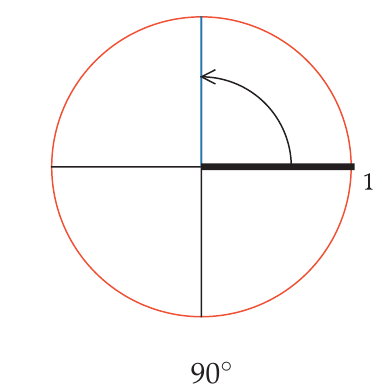
\includegraphics[scale=0.5]{1.png}

\end{frame}

\begin{frame}
    \frametitle{Radius corresponding to a negative angle}
    \centering
    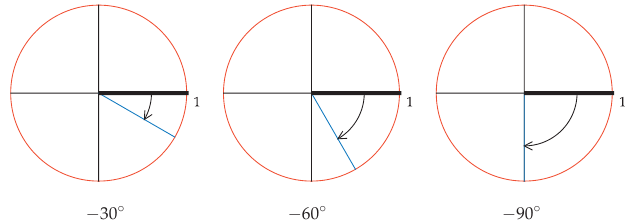
\includegraphics[scale=0.5]{2.png}

\end{frame}

\begin{frame}
    \begin{block}{Positive and Negative Angles}
        \begin{itemize}
            \item Angle measurements for a radius on the unit circle are made from the
            positive horizontal axis.
            \item Positive angles correspond to moving counterclockwise from the positive
            horizontal axis.
            \item Negative angles correspond to moving clockwise from the positive hori-
            zontal axis.
        \end{itemize}
    \end{block}
\end{frame}

\begin{frame}
    \begin{figure}[h]    
        \begin{minipage}[b]{0.3\textwidth}
        \centering
        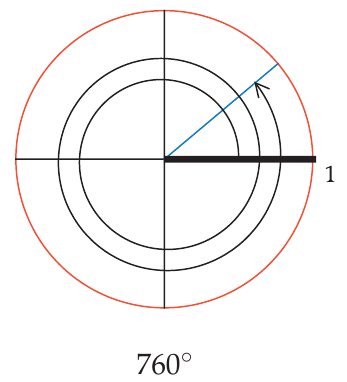
\includegraphics[scale=0.25]{3.png}
        \caption{+ve angle}
    \end{minipage}
    \begin{minipage}[b]{0.3\textwidth}
        \centering
        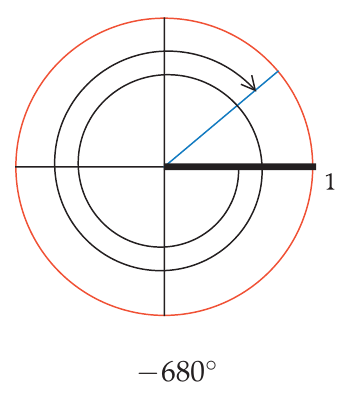
\includegraphics[scale=0.25]{4.png}
        \caption{-ve angle}
    \end{minipage}
\end{figure}
\begin{block}{cyclic hehaviour of angles}
    A radius of the unit circle corresponding to $\theta$ degrees also corresponds to
$\theta + 360n$ degrees for every integer n.
\end{block}
\end{frame}


\begin{frame}
    \frametitle{Length of a Circular Arc}
    \centering
    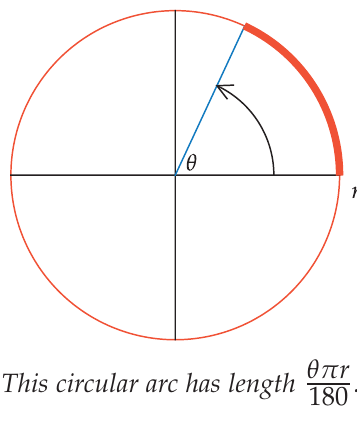
\includegraphics[scale=0.5]{5.png}
\end{frame}

\begin{frame}
    \frametitle{Radians}
   \begin{block}{Radians}
    Radians are a unit of measurement for angles such that $2\pi$ radians correspond
    to a rotation through an entire circle.
   \end{block}
\end{frame}

\begin{frame}
    \frametitle{Radians}
    \centering
    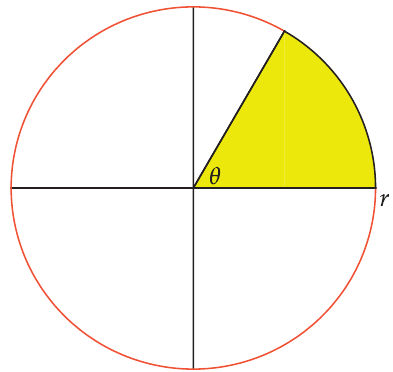
\includegraphics[scale=0.3]{6.png}
\end{frame}
\begin{frame}
    \frametitle{Radians}
   \begin{block}{Degree to Radians}

    $$ 360^{\circ} = 2 \pi radians $$
    $$ 1 ^{\circ}  = \frac{2 \pi}{360} radians $$
    
   \end{block}
\end{frame}

\begin{frame}
    \frametitle{Arc Length}
    \begin{block}{length of a circular arc}
        If $0 < \theta \leq 2\pi$ , then a circular arc on the unit circle corresponding to $\theta$ radians
        has length $\theta$         
    \end{block}
\end{frame}

\begin{frame}
        \begin{figure}[h]    
            \begin{minipage}[b]{0.3\textwidth}
            \centering
            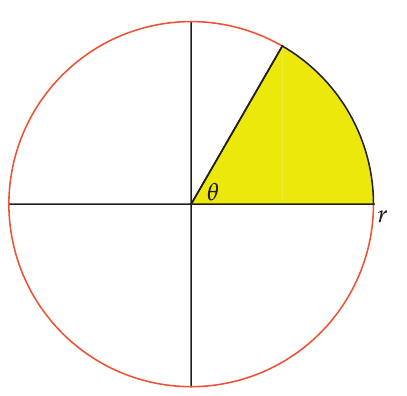
\includegraphics[scale=0.25]{7.png}
            \caption{Area of slice}
        \end{minipage}
    \end{figure}
    \begin{block}{Area of slice}
        A slice with angle $\theta$ radians inside a circle with radius $r$ has area $\frac{1}{2} \theta r^{2}$ .
    \end{block}
\end{frame}

\begin{frame}
    \frametitle{Cosine and Sine}
    \begin{figure}[h]    
        \begin{minipage}[b]{0.8\textwidth}
        \centering
        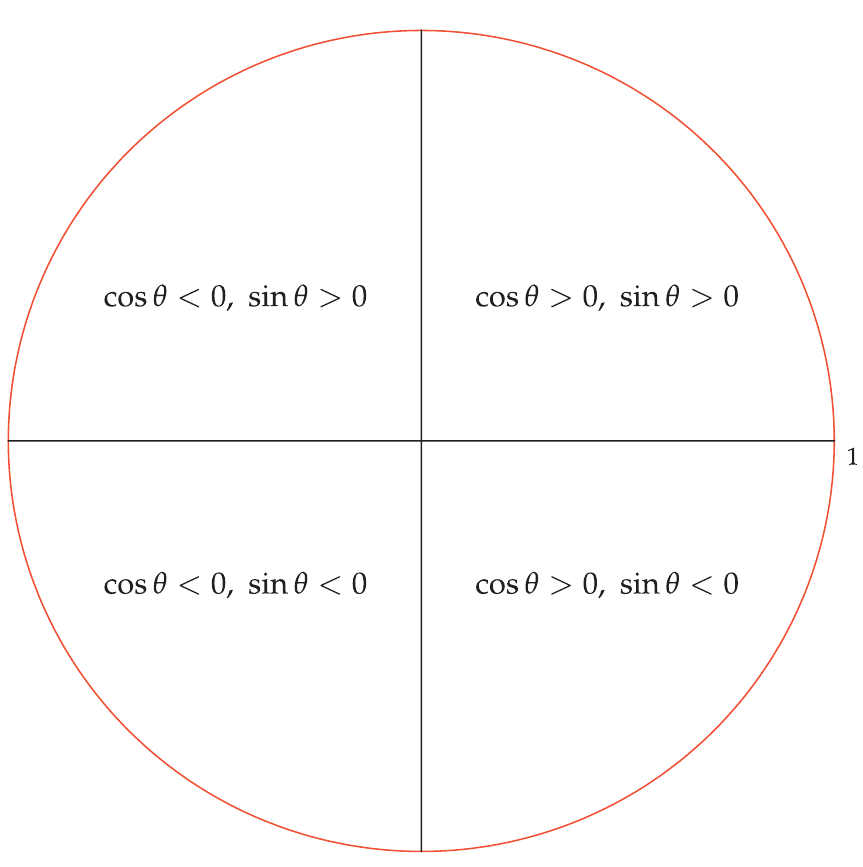
\includegraphics[scale=0.22]{8.png}
        \caption{sin and cos}
    \end{minipage}
\end{figure}
\end{frame}
\end{document}